% generated by make_combined.py from stage9_remedies_dominance/stage9.tex; do not edit
\section{Stage 9 --- Is there a remedy that beats masking everywhere?}\label{sec:stage9}

\stagebox{\textbf{In one sentence.} No remedy dominates ROI masking --- none of the seven candidates registered in two rounds
(four, then three chosen by a search over twelve ideas) is never worse and better wherever masking fails --- but the best
ones come within one cell: a
class-conditional mean constraint on the masked features (\texttt{mask\_cmc}) and IRMv1 are better than masking in every
Trap~A (including a cohort held out from all choices) and on the shortcut-conflicting cases of every unaltered test set,
equal to it elsewhere, and lose only on the external ISIC 2020 set (\sNineCmcDOneallisicTwoZeroTwoZero{} and
\sNineNinemaskirmDOneisicTwoZeroTwoZero{} overall AUROC), where every alternative to masking, including the unmasked
model, loses.}
\subsection{Where this stage starts}
Stage~6 developed and compared remedies for the failure of masking and concluded that the right remedy depends on what
carries the shortcut, and that no remedy improved on masking uniformly on unaltered data. Stage~8 validated the labels
the remedies need and showed the failure on a near-benchmark model. One question remained: is there \emph{one} method a
practitioner could use instead of masking --- never worse, and better where masking fails? This stage answers it with a
registered criterion, two registered rounds on data generated only after each registration, and a documented search
between them.

\subsection{Questions}
\begin{enumerate}[label=\textbf{Q9\alph*},leftmargin=*]\itemsep1pt
\item Does any existing or adapted remedy dominate masking by a registered criterion?
\item If not, where exactly does the best one lose, and why?
\item Can a search over further ideas, including methods from outside medical imaging, find one that does?
\end{enumerate}
\paragraph{Design decisions} \emph{The comparison is with masking only.} ``Dominates'' means not worse where masking
already works and better where it fails (Table~\ref{s9:tab:crit}); it does not require beating every other remedy.
\emph{Cells where no honest method can win are left out}: easy pairs (a method that stops using the shortcut must lose
there) and correlated tests as strong as training (the criterion uses the worse of the reversed and correlated tests).
\emph{One criterion, many components.} A candidate dominates only if all 42 components are met (an intersection--union
test, so no correction within a candidate); across candidates a fixed sequence, registered in advance, keeps the full
0.025 for the first. \emph{Choices on validation data only.} Every setting is chosen per training set by the worst-group
validation AUROC with a guard on the same-artifact pairs, which measure disease ranking whatever the association; masking
is always a fallback. \emph{Untouched confirmation.} New trap resamples with seeds used for nothing else, and one cohort
(ovary) whose data never influence a choice. The unaltered test sets and ISIC 2020 had been seen before and are
semi-confirmatory. \emph{Novelty is not a condition}: every candidate is labelled published or adaptation with its closest
prior work; none is new. \emph{At deployment} a candidate may use only the image, its ROI mask and automatic detectors.

\subsection{Methods}
\paragraph{Design (no test scoring)} Every existing arm was recomputed on one crossed bootstrap (11{,}135 cells); the
closest existing arm met 29 of 36 cells of the criterion. An exact decomposition of the all-pairs AUROC into easy,
conflicting and same-artifact pairs showed that balancing loses on unaltered data mainly through the same-artifact
pairs, i.e.\ through disease signal lost by reweighting, not through removing the shortcut.
\paragraph{Round 8 candidates} (i) \texttt{mask\_cmc}: masked features projected onto the complement of the within-class
mean differences between images with and without the artifact, so the head may not score them differently on average
within a class; a first-moment, linear case of counterfactual invariance (Veitch et al.\ 2021). (ii) \texttt{full\_cmc}:
the same on the full image. (iii) \texttt{mask\_bal}: partial group reweighting with a validated strength. (iv)
\texttt{locrand\_loc}: real artifact instances pasted inside and outside the ROI so that presence at each location is
independent of the label. Nine further arms (the uniform paste plan, a selector, combinations, AFR, GroupDRO, a soft U-MtE, a label-sensitivity run) are descriptive.
Separate claims: controlled sweeps (D5), a fine-tuned paste model (D6), replication with MedSigLIP and ConvNeXt (R).
One amendment, before any run, replaced Holm across candidates by the fixed sequence, made the location-matched paste
plan primary and labelled failed components as \emph{loss} or \emph{inconclusive}.
\paragraph{Search} After round 8, twelve ideas were tried on development data only (development seeds; validation folds
of the unaltered training sets; never a confirmation seed, test set, ISIC 2020 or ovary; enforced in code): backdoor
adjustment, product of experts and logit adjustment from NLP and long-tail learning, moment matching, conditional
adversarial debiasing, Correct-n-Contrast and counterfactual contrastive learning, V-REx and IRMv1, and combinations.
Every attempt is logged.
\paragraph{Round 9} The three best eligible search candidates, in the fixed sequence conditional adversarial debiasing
$\to$ IRMv1 $\to$ V-REx, with round 8's \texttt{mask\_cmc} and \texttt{mask\_bal} refitted with their frozen recipes as
references; new confirmation seeds; registered as the last remedy round.

\subsection{Experiments}
\begin{table}[H]\centering\scriptsize
\caption{Experiments of this stage. Each registration was committed before the data it tests were generated (round 8: confirmation seeds 8101--8505; round 9: 9101--9505). Commit times are set by the committing machine.}\label{s9:tab:exp}
\begin{tabular}{p{5.0cm}p{3.6cm}p{2.8cm}p{3.6cm}}\toprule
Experiment & Status & First commit (local time) & Support criterion \\\midrule
Design and scoreboard of every existing arm & \posthoc{design; no test scoring of new models} & \texttt{86e99d8}, 2026-09-28 21:19 & -- \\
Round 8: four primary candidates (fixed sequence), sweeps (D5), fine-tuned (D6), replication (R) & \registered{round 8}; one amendment before any run & \texttt{dd5c7ee}, 2026-09-28 22:01 & dominance: every component of D1--D4 met (intersection--union) \\
Search over twelve candidates on development data & \posthoc{exploratory; development data only} & \texttt{8645734}, 2026-09-29 00:15 & ranking only \\
Round 9: three candidates from the search (fixed sequence) & \registered{round 9}; the last remedy round & \texttt{6563a66}, 2026-09-29 08:44 & as round 8 \\
\bottomrule\end{tabular}
\end{table}

\begin{table}[H]\centering\scriptsize
\caption{The registered criterion for ``dominates masking''. A candidate dominates only if every component is met; easy pairs, where any method that stops using the shortcut must lose, are not in it.}\label{s9:tab:crit}
\begin{tabular}{lp{9.0cm}p{5.0cm}}\toprule
 & Cells & Test (candidate $-$ masking, one-sided 0.025) \\\midrule
D1 & all pairs of the six unaltered test sets (thyroid split, capsule, BCN, HAM, MSK, ISIC 2019 $\to$ 2020) & not worse: lower bound $>-0.01$ \\
D2 & shortcut-conflicting pairs (thyroid, BCN, MSK, ISIC 2020) and Trap~A $\min$(reversed, correlated) in four cohorts & better: lower bound $>0$ \\
D3 & Trap~B and clean tests, per cell (16) and pooled over cohorts (4) & not worse: $-0.03$ per cell, $-0.01$ pooled \\
D4 & every trap & no shortcut flipping: correlated $\ge$ reversed $-0.02$ \\
\bottomrule\end{tabular}
\end{table}


\subsection{Results}
\subsubsection{Round 8: close, but no dominance}
Table~\ref{s9:tab:rEight}. The sequence stopped at its first candidate: \texttt{mask\_cmc} met \sNineMetmaskcmc{} of
\sNineNComp{} components. It is better than masking in every Trap~A --- thyroid \sNineCmcDTwoTrapthyroid, capsule
\sNineCmcDTwoTrapcapsule, dermoscopy hair \sNineCmcDTwoTrapisic{} and the held-out ovary \sNineCmcDTwoTrapovary{} --- and
on the conflicting pairs of every unaltered test set, including ISIC 2020 (\sNineCmcDTwohardisicTwoZeroTwoZero); it is not
worse on Trap~B and the clean tests, never flips the shortcut, and is not worse overall on four of the six unaltered test
sets (thyroid inconclusive: \sNineCmcDOneallthyroid). Its one loss is ISIC 2020 overall (\sNineCmcDOneallisicTwoZeroTwoZero).
\texttt{mask\_bal} also met every D2 component but lost small amounts overall on thyroid, MSK and ISIC 2020
(Table~\ref{s9:tab:rEightc}, Figure~\ref{s9:fig:dom}).
\begin{table}[H]\centering\scriptsize
\caption{Round 8 on the confirmation data: no candidate dominates masking. The sequence stopped at its first candidate; the others are reported unadjusted.}\label{s9:tab:rEight}
\begin{tabular}{p{4.6cm}p{1.6cm}p{1.3cm}p{5.0cm}p{2.6cm}}\toprule
Candidate & Components met & All of D2 met & Losses & Fixed sequence \\\midrule
class-conditional mean constraint (\texttt{mask\_cmc}) & 40 of 42 & yes & ISIC 2019 $\to$ 2020 (D1) & tested, not rejected \\
mean constraint on the full image (\texttt{full\_cmc}) & 36 of 42 & no & dermoscopy, HAM held out (D1), dermoscopy, MSK held out (D1), ISIC 2019 $\to$ 2020 (D1) & not tested in the sequence \\
partial reweighting (\texttt{mask\_bal}) & 39 of 42 & yes & thyroid split (D1), dermoscopy, MSK held out (D1), ISIC 2019 $\to$ 2020 (D1) & not tested in the sequence \\
location-matched pasting (\texttt{locrand\_loc}) & 39 of 42 & no & dermoscopy, BCN held out (D2) & not tested in the sequence \\
\bottomrule\end{tabular}
\end{table}

\begin{table}[H]\centering\scriptsize
\caption{Round 8, the two candidates that won everywhere masking fails: the D1 and D2 components and the pooled D3 components (AUROC, crossed 95\% CIs); every per-cell D3 component and D4 were met by both.}\label{s9:tab:rEightc}
\begin{tabular}{p{2.3cm}p{3.3cm}p{2.9cm}p{1.4cm}p{2.9cm}p{1.4cm}}\toprule
Component & Cell & \texttt{mask\_cmc} $-$ masking &  & \texttt{mask\_bal} $-$ masking &  \\\midrule
D1 all pairs & thyroid split & $-0.002$ [$-0.011, +0.007$] & inconclusive & $-0.008$ [$-0.017, +0.001$] & \textbf{loss} \\
D1 all pairs & capsule & $-0.000$ [$-0.001, +0.001$] & met & $-0.001$ [$-0.004, +0.000$] & met \\
D1 all pairs & dermoscopy, BCN held out & $-0.005$ [$-0.006, -0.003$] & met & $+0.003$ [$+0.000, +0.007$] & met \\
D1 all pairs & dermoscopy, HAM held out & $-0.003$ [$-0.008, +0.002$] & met & $+0.003$ [$-0.001, +0.008$] & met \\
D1 all pairs & dermoscopy, MSK held out & $-0.002$ [$-0.006, +0.002$] & met & $-0.006$ [$-0.011, -0.000$] & \textbf{loss} \\
D1 all pairs & ISIC 2019 $\to$ 2020 & $-0.021$ [$-0.027, -0.016$] & \textbf{loss} & $-0.011$ [$-0.016, -0.005$] & \textbf{loss} \\
D2 conflicting pairs & thyroid split & $+0.084$ [$+0.069, +0.101$] & met & $+0.048$ [$+0.032, +0.066$] & met \\
D2 conflicting pairs & dermoscopy, BCN held out & $+0.036$ [$+0.033, +0.040$] & met & $+0.033$ [$+0.026, +0.040$] & met \\
D2 conflicting pairs & dermoscopy, MSK held out & $+0.070$ [$+0.059, +0.082$] & met & $+0.044$ [$+0.030, +0.058$] & met \\
D2 conflicting pairs & ISIC 2019 $\to$ 2020 & $+0.078$ [$+0.069, +0.088$] & met & $+0.035$ [$+0.024, +0.046$] & met \\
D2 Trap~A & thyroid & $+0.330$ [$+0.311, +0.351$] & met & $+0.380$ [$+0.355, +0.404$] & met \\
D2 Trap~A & capsule & $+0.153$ [$+0.131, +0.177$] & met & $+0.166$ [$+0.148, +0.185$] & met \\
D2 Trap~A & ovary (held out) & $+0.118$ [$+0.089, +0.147$] & met & $+0.161$ [$+0.135, +0.187$] & met \\
D2 Trap~A & dermoscopy hair & $+0.193$ [$+0.166, +0.221$] & met & $+0.213$ [$+0.187, +0.239$] & met \\
D3 pooled & Trap B reversed & $+0.020$ [$+0.014, +0.026$] & met & $+0.045$ [$+0.036, +0.054$] & met \\
D3 pooled & clean (Trap A models) & $+0.057$ [$+0.048, +0.065$] & met & $+0.063$ [$+0.054, +0.072$] & met \\
D3 pooled & clean (Trap B models) & $+0.007$ [$+0.002, +0.012$] & met & $+0.010$ [$+0.002, +0.017$] & met \\
\bottomrule\end{tabular}
\end{table}

\paragraph{Why ISIC 2020} On ISIC 2020 in-lesion hair still points towards melanoma for most patients. \texttt{mask\_cmc}
removes that shortcut: it gains \sNineCmcIsicTwoZerohard{} on the conflicting pairs and loses \sNineCmcIsicTwoZeroeasy{} on
the easy pairs, where the shortcut gives the right answer; the rest of the overall loss comes from the same-artifact
pairs.
\paragraph{Separate claims} In the controlled sweeps \texttt{mask\_cmc} and \texttt{mask\_bal} dominate masking
(\sNineDFivemaskcmc{} components each; D5, Holm). The replication with MedSigLIP and ConvNeXt supports the Trap~A gain in
\sNineRepmaskcmc{} cohorts for \texttt{mask\_cmc} (smallest gain \sNineRepMinmaskcmc) and \sNineRepmaskbal{} for
\texttt{mask\_bal}. The paste candidates are not a fair test: in the traps too few images could receive a paste to balance
presence between the classes, and a probe separates pasted from real artifacts (AUROC \sNineProbeMin--\sNineProbeMax); the
fine-tuned paste model met \sNineDSix{} components (D6).

\subsubsection{The search}
Table~\ref{s9:tab:search}. None of the \sNineNSearch{} candidates met every development component. Three flip the shortcut in
thyroid Trap~A and are not eligible (backdoor adjustment, product of experts, logit adjustment); the contrastive methods
lose disease signal. The three kept met 27--28 of 29 with no loss --- but round 8's \texttt{mask\_bal} also scored
\sNineSearchBal{} of 29 on this development criterion and still lost on ISIC 2020, which the search could not see.
\begin{table}[H]\centering\scriptsize
\caption{The exploratory search: twelve candidates on development data only (development seeds, validation folds of the unaltered training sets; never a test set used for confirmation, never ovary). Round 8's candidates are shown on the same development criterion for comparison.}\label{s9:tab:search}
\begin{tabular}{p{5.4cm}p{2.4cm}p{1.0cm}p{2.8cm}p{2.2cm}}\toprule
Search candidate (frozen masked features) & Development components met & Losses & Eligible & Registered in round 9 \\\midrule
backdoor adjustment & 22 of 29 & 6 & no (flips the shortcut) & -- \\
backdoor adjustment, full image & 22 of 29 & 1 & yes & -- \\
constraint + backdoor & 23 of 29 & 4 & yes & -- \\
constraint + backdoor, full image & 23 of 29 & 1 & yes & -- \\
product of experts & 28 of 29 & 1 & no (flips the shortcut) & -- \\
group logit adjustment & 28 of 29 & 1 & no (flips the shortcut) & -- \\
moment matching & 26 of 29 & 1 & yes & -- \\
conditional adversarial debiasing & 27 of 29 & 0 & yes & 1st \\
Correct-n-Contrast & 20 of 29 & 3 & yes & -- \\
counterfactual contrastive & 19 of 29 & 4 & yes & -- \\
V-REx & 28 of 29 & 0 & yes & 3rd \\
IRMv1 & 28 of 29 & 0 & yes & 2nd \\
round 8 \texttt{mask\_cmc} (reference) & 27 of 29 & 1 & yes & -- \\
round 8 \texttt{mask\_bal} (reference) & 28 of 29 & 0 & yes & -- \\
\bottomrule\end{tabular}
\end{table}


\subsubsection{Round 9: the same result on new data}
Table~\ref{s9:tab:rNine} and Figure~\ref{s9:fig:dom}. Conditional adversarial debiasing, first in the sequence, met only
\sNineNineMetmaskcondadv{} components; the sequence stopped. IRMv1 met \sNineNineMetmaskirm, losing only ISIC 2020 overall
(\sNineNinemaskirmDOneisicTwoZeroTwoZero, just beyond the margin of $-0.01$) while gaining on its conflicting pairs
(\sNineNinemaskirmDTwoisicTwoZeroTwoZero); V-REx met \sNineNineMetmaskvrex. Refitted on the new data with its frozen recipe,
\texttt{mask\_cmc} met \sNineNineMetmaskcmc{} and again lost only ISIC 2020 overall (\sNineNinemaskcmcDOneisicTwoZeroTwoZero):
the round-8 result replicates. IRMv1 gains less than \texttt{mask\_cmc} where masking fails (Table~\ref{s9:tab:rNineg}), so it
sits at a different point of the same trade-off.
\begin{table}[H]\centering\scriptsize
\caption{Round 9 on new confirmation data (seeds 9101--9505): no candidate dominates masking. Round 8's two best candidates, refitted with their frozen recipes, are descriptive references on the same data.}\label{s9:tab:rNine}
\begin{tabular}{p{4.6cm}p{1.6cm}p{1.3cm}p{5.2cm}p{2.4cm}}\toprule
Candidate & Components met & All of D2 met & Losses & Role \\\midrule
conditional adversarial debiasing (\texttt{mask\_condadv}) & 27 of 42 & no & dermoscopy, MSK held out (D1), ISIC 2019 $\to$ 2020 (D1), ovary (held out) (D3), ovary (held out) (D3), ovary (held out) (D3), thyroid+capsule+ovary+isic (D3) & tested, not rejected \\
IRMv1 (\texttt{mask\_irm}) & 41 of 42 & yes & ISIC 2019 $\to$ 2020 (D1) & not tested in the sequence \\
V-REx (\texttt{mask\_vrex}) & 40 of 42 & yes & ISIC 2019 $\to$ 2020 (D1) & not tested in the sequence \\
class-conditional mean constraint (\texttt{mask\_cmc}) & 41 of 42 & yes & ISIC 2019 $\to$ 2020 (D1) & reference (round 8) \\
partial reweighting (\texttt{mask\_bal}) & 38 of 42 & yes & thyroid split (D1), dermoscopy, MSK held out (D1), ISIC 2019 $\to$ 2020 (D1) & reference (round 8) \\
\bottomrule\end{tabular}
\end{table}

\begin{table}[H]\centering\scriptsize
\caption{Round 9: gains over masking where masking fails (Trap~A $\min$(reversed, correlated); conflicting pairs), crossed 95\% CIs.}\label{s9:tab:rNineg}
\resizebox{\linewidth}{!}{\begin{tabular}{lcccc}\toprule
Where masking fails & IRMv1 & V-REx & \texttt{mask\_cmc} (ref.) & \texttt{mask\_bal} (ref.) \\\midrule
thyroid & $+0.229$ [$+0.205, +0.255$] & $+0.322$ [$+0.303, +0.343$] & $+0.333$ [$+0.314, +0.353$] & $+0.393$ [$+0.363, +0.414$] \\
capsule & $+0.030$ [$+0.008, +0.053$] & $+0.156$ [$+0.135, +0.181$] & $+0.143$ [$+0.118, +0.172$] & $+0.164$ [$+0.140, +0.189$] \\
ovary (held out) & $+0.057$ [$+0.037, +0.080$] & $+0.081$ [$+0.055, +0.108$] & $+0.094$ [$+0.066, +0.122$] & $+0.134$ [$+0.101, +0.170$] \\
dermoscopy hair & $+0.120$ [$+0.096, +0.143$] & $+0.193$ [$+0.170, +0.216$] & $+0.205$ [$+0.181, +0.229$] & $+0.218$ [$+0.194, +0.245$] \\
conflicting pairs, thyroid split & $+0.049$ [$+0.030, +0.073$] & $+0.088$ [$+0.061, +0.114$] & $+0.062$ [$+0.030, +0.088$] & $+0.046$ [$+0.030, +0.063$] \\
conflicting pairs, dermoscopy, BCN held out & $+0.017$ [$+0.013, +0.022$] & $+0.022$ [$+0.020, +0.025$] & $+0.037$ [$+0.034, +0.039$] & $+0.028$ [$+0.021, +0.035$] \\
conflicting pairs, dermoscopy, MSK held out & $+0.036$ [$+0.025, +0.048$] & $+0.059$ [$+0.050, +0.067$] & $+0.055$ [$+0.026, +0.078$] & $+0.049$ [$+0.038, +0.060$] \\
conflicting pairs, ISIC 2019 $\to$ 2020 & $+0.028$ [$+0.022, +0.035$] & $+0.043$ [$+0.037, +0.050$] & $+0.056$ [$+0.026, +0.079$] & $+0.039$ [$+0.030, +0.048$] \\
\bottomrule\end{tabular}}
\end{table}

\paragraph{ISIC 2020 is where masking itself is strong} Table~\ref{s9:tab:decomp}. Every arm loses there overall, from
\sNineDecBest{} to \sNineDecWorst{} --- including the unmasked model (ERM, \sNineDecErm), whose loss comes mostly from the
same-artifact pairs (\sNineDecErmSame). On new patients at natural prevalence, masking ranks disease better than any
alternative we tested, and a method that removes the in-lesion hair shortcut additionally gives up the easy pairs.
\begin{table}[H]\centering\scriptsize
\caption{ISIC 2019 $\to$ 2020, round 9: the all-pairs difference to masking split exactly into the contributions of the pair types (share of pairs $\times$ difference). Every arm, including the unmasked model (ERM), loses mostly on the same-artifact pairs, i.e.\ disease ranking, not only on the easy pairs.}\label{s9:tab:decomp}
\begin{tabular}{lcccc}\toprule
Arm & Easy pairs & Conflicting pairs & Same-artifact pairs & All pairs \\\midrule
erm & -0.005 & 0.002 & -0.010 & -0.014 \\
mask\_bal & -0.007 & 0.002 & -0.010 & -0.015 \\
mask\_cmc & -0.011 & 0.003 & -0.007 & -0.015 \\
mask\_condadv & -0.006 & 0.000 & -0.024 & -0.029 \\
mask\_irm & -0.005 & 0.002 & -0.005 & -0.009 \\
mask\_vrex & -0.009 & 0.002 & -0.006 & -0.012 \\
\bottomrule\end{tabular}
\end{table}

\begin{figure}[H]\centering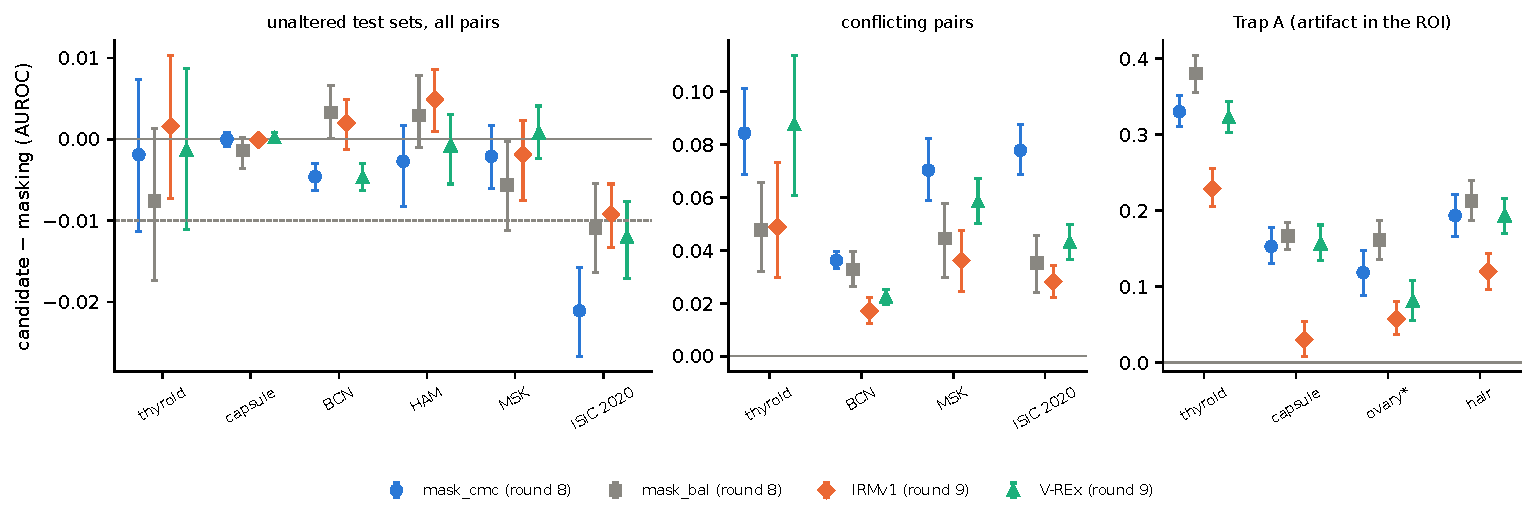
\includegraphics[width=\linewidth]{../stage9_remedies_dominance/figures/dominance.pdf}
\caption{The four best candidates minus masking (crossed 95\% CIs). Left: all pairs of the unaltered test sets (dashed:
the registered margin $-0.01$). Middle: conflicting pairs. Right: Trap~A $\min$(reversed, correlated); *ovary held out from
every choice.}\label{s9:fig:dom}\end{figure}

\subsection{What failed or changed}
\begin{itemize}[leftmargin=*]\itemsep1pt
\item \textbf{No dominance} in either round; the best candidates fail on one cell, ISIC 2020 overall.
\item \textbf{The paste candidates} were not a fair test (too few recipients to balance the traps; pasted artifacts
distinguishable from real ones).
\item \textbf{The development criterion} of the search could not see ISIC 2020; the candidate it ranked first (conditional
adversarial debiasing) failed most in confirmation.
\item \textbf{A premise in the approval of round 8 was wrong}: the trap validation split does not carry the training
association. The registered guard was kept because it is right either way.
\item \textbf{Scope}: frozen DINOv2 features for the dominance test; replication in two encoders for Trap~A only; the
fine-tuned route (D6) was tested only with the paste candidate.
\end{itemize}

\subsection{Anticipated questions}
\paragraph{Is a loss of 0.01--0.02 AUROC on one external set a reason to keep masking?} It is a trade-off, not a
verdict. \texttt{mask\_cmc} gives up \sNineCmcDOneallisicTwoZeroTwoZero{} overall on ISIC 2020 and gains
\sNineCmcDTwohardisicTwoZeroTwoZero{} on the cases in which the shortcut points the wrong way, and it removes masking's
failure wherever the artifact lies inside the ROI. Which matters more is a clinical choice; the registered criterion
counts the overall loss as a failure, and we report it as one.
\paragraph{Why was the criterion so strict?} Because ``better than masking'' is only useful if it holds everywhere a user
might deploy the method. The strictness also makes the negative result informative: the candidates fail by one cell, not
by many.
\paragraph{Were twelve search candidates a fishing expedition?} The search used development data only, every attempt is
logged with its prediction, and the three candidates it produced were confirmed on data generated after their
registration --- where they did not dominate.
\paragraph{Is \texttt{mask\_cmc} new?} No. It is an adaptation of counterfactual invariance (a class-conditional
constraint) applied after masking; what is new is deriving it from the location law and the pair decomposition, and
testing it this way.
\paragraph{Why does even the unmasked model lose on ISIC 2020?} Masking is strong there: the unmasked model loses mostly
on the same-artifact pairs, i.e.\ it ranks disease worse when the surroundings are kept, presumably because skin context
and hair beside the lesion transfer poorly between the two collections. That is consistent with the location law ---
masking helps where the shortcut lies outside the ROI --- and it explains why an alternative that keeps context, or that
also removes the in-lesion shortcut, falls short of masking overall on this set.

\subsection{Conclusion}
\textbf{Not supported.} No remedy dominates masking (seven registered candidates in rounds 8 and 9; twelve searched).
\textbf{Supported, as a trade-off.} A class-conditional mean constraint on masked features, and IRMv1, are better than
masking wherever masking fails --- every Trap~A including a held-out cohort, the conflicting cases of every unaltered test
set --- and equal to it elsewhere, except for a loss of 0.01--0.02 overall AUROC on the external ISIC 2020 set, where
every alternative to masking loses. In the controlled sweeps both round-8 winners dominate masking.

\subsection{Questions for the supervisor}
\begin{enumerate}\itemsep1pt
\item Should the paper recommend \texttt{mask\_cmc} as the remedy to use when artifacts may lie inside the ROI,
stating its ISIC 2020 cost, or only report it?
\item Should the negative dominance result (two registered rounds) enter the main text, as the answer to ``so what should
we use instead?''?
\item Is closing the remedy question here --- no further search --- acceptable?
\end{enumerate}

